\documentclass[twocolumn]{aastex631}

\usepackage{graphicx}
\usepackage{amsmath}

\shorttitle{A Mars--Earth Grazing Collision Visualization}
\shortauthors{Laughlin}

\begin{document}

\title{A Smoothed-Particle Hydrodynamics Visualization of a Grazing Mars--Earth Collision}

\author{Gregory Laughlin}

\begin{abstract}
We describe a numerical and rendering workflow for a near-grazing collision
between differentiated Earth- and Mars-mass bodies.  The calculation was
developed to support a scientific visualization of Solar System instability
outcomes, rather than to establish a converged impact outcome.  Initial bodies
are generated with WoMa, relaxed in SWIFT, assembled on a grazing trajectory,
and evolved with self-gravity and hydrodynamics.  Surface tracer particles are
advected with the flow and colored to indicate terrestrial land/ocean material
and the Mars impactor.  The high-resolution calculation begins with 218,271 SPH
particles, an impact angle of 70 degrees from head-on, and a contact velocity of
1.02 times the mutual escape speed.  It has been evolved through 92 simulated
hours, with 215,299 particles present in the final snapshot.  The calculation
shows strong tidal deformation and stripping during the initial grazing passage,
followed by a second finite-size encounter and an extended debris stream.  The
available calculation does not yet establish the final binding hierarchy.  We
emphasize the
distinction between this presentation-quality simulation product and a
publication-quality convergence study: future work must quantify energy and
angular-momentum conservation, equation-of-state sensitivity, resolution
dependence, and outcome boundaries in velocity-angle-impact-parameter space.
\end{abstract}

\keywords{Hydrodynamical simulations (767) --- Impact phenomena (779) ---
Terrestrial planets (1708) --- Planetary collisions (2203)}

\section{Introduction}

The long-term stability of terrestrial planetary systems is punctuated, in
some regions of parameter space, by close encounters and direct collisions.
For public and scientific presentations, these events are difficult to convey
with point-mass integrations alone: the dynamical encounter is driven by
orbital mechanics, but the memorable observable consequence is a material
process involving tidal distortion, ejecta, accretion, and possible survival of
a coherent remnant.  The present project builds a reproducible local workflow
for visualizing one such event, a grazing encounter between Earth- and
Mars-mass bodies.

The calculation is not intended as a claim that a specific Mars--Earth impact
is likely in the present Solar System, nor as a converged prediction for the
outcome of any particular instability scenario.  Instead, it provides a
scientifically grounded animation: the bodies are differentiated, self-gravity
is active, material surfaces are advected as tracers, and the rendering is tied
to the actual SPH particle state.  This document records the numerical setup,
the rendering strategy, and the limitations that separate the current product
from a peer-reviewed impact-outcome survey.

\section{Numerical Setup}

The initial conditions are generated with WoMa and evolved with SWIFT.  The
target has approximately Earth mass and radius, while the impactor has
approximately Mars mass and radius.  Both bodies are differentiated
iron-silicate objects using ANEOS Fe85Si15 and forsterite material tables.
Separate Earth and Mars bodies are first relaxed, then assembled into an impact
configuration.

The main calculation uses a requested resolution of
$N_{\rm total}=200{,}000$, yielding 218,271 particles after shell population
adjustment.  The nominal impact geometry is a 70 degree angle from head-on, with
an initial contact speed of $1.02\,v_{\rm esc}$, where $v_{\rm esc}$ is the
two-body mutual escape speed.  The trajectory is initialized about two hours
before nominal contact and is evolved in stages through 92 hours.  The final
snapshot contains 215,299 particles; this loss of particle IDs must be audited
explicitly in any conservation or mass-partition analysis.  Exact configuration
files and compact continuation inputs are included in the repository.  The
multi-gigabyte snapshot series and continuation logs remain in the documented
external SWIFT working tree.

\section{Rendering Method}

Visualization is performed from the SPH particle snapshots.  Each particle is
matched to a sidecar label file by its \texttt{ParticleIDs} value.  Label files
store the source body, surface class, longitude/latitude at initialization, and
RGB colors.  The Earth surface colors represent a coarse present-day
land/ocean pattern, with a rendering-only coastline refinement that demotes
continental-shelf-adjacent particles from land to ocean for a cleaner visual
map.  The Mars colors use a procedural albedo pattern intended to evoke the
global appearance of Mars, including ochre dust, darker basaltic provinces, and
subtle polar frost.

The early direct-view movie is rendered in an inertial frame with bounds chosen
from robust Earth and Mars extents.  The longer presentation movie uses a wider
fixed global frame so that the main remnant and debris stream remain visible
through the second encounter.  The renderer intersects persistent particle IDs
over each selected snapshot sequence.  Surface tracers are drawn as crisp
depth-sorted points over a dim body-base layer, while the storyboard and
density-trial renderers provide alternative views for presentation work.  The
current long-form presentation cut reaches approximately 89 hours; the final
three simulated hours exist in the snapshot archive but are not included in that
movie.

\begin{figure*}[t]
\centering

\includegraphics[width=0.49\textwidth]{../docs/figures/direct_view_00_start.png}
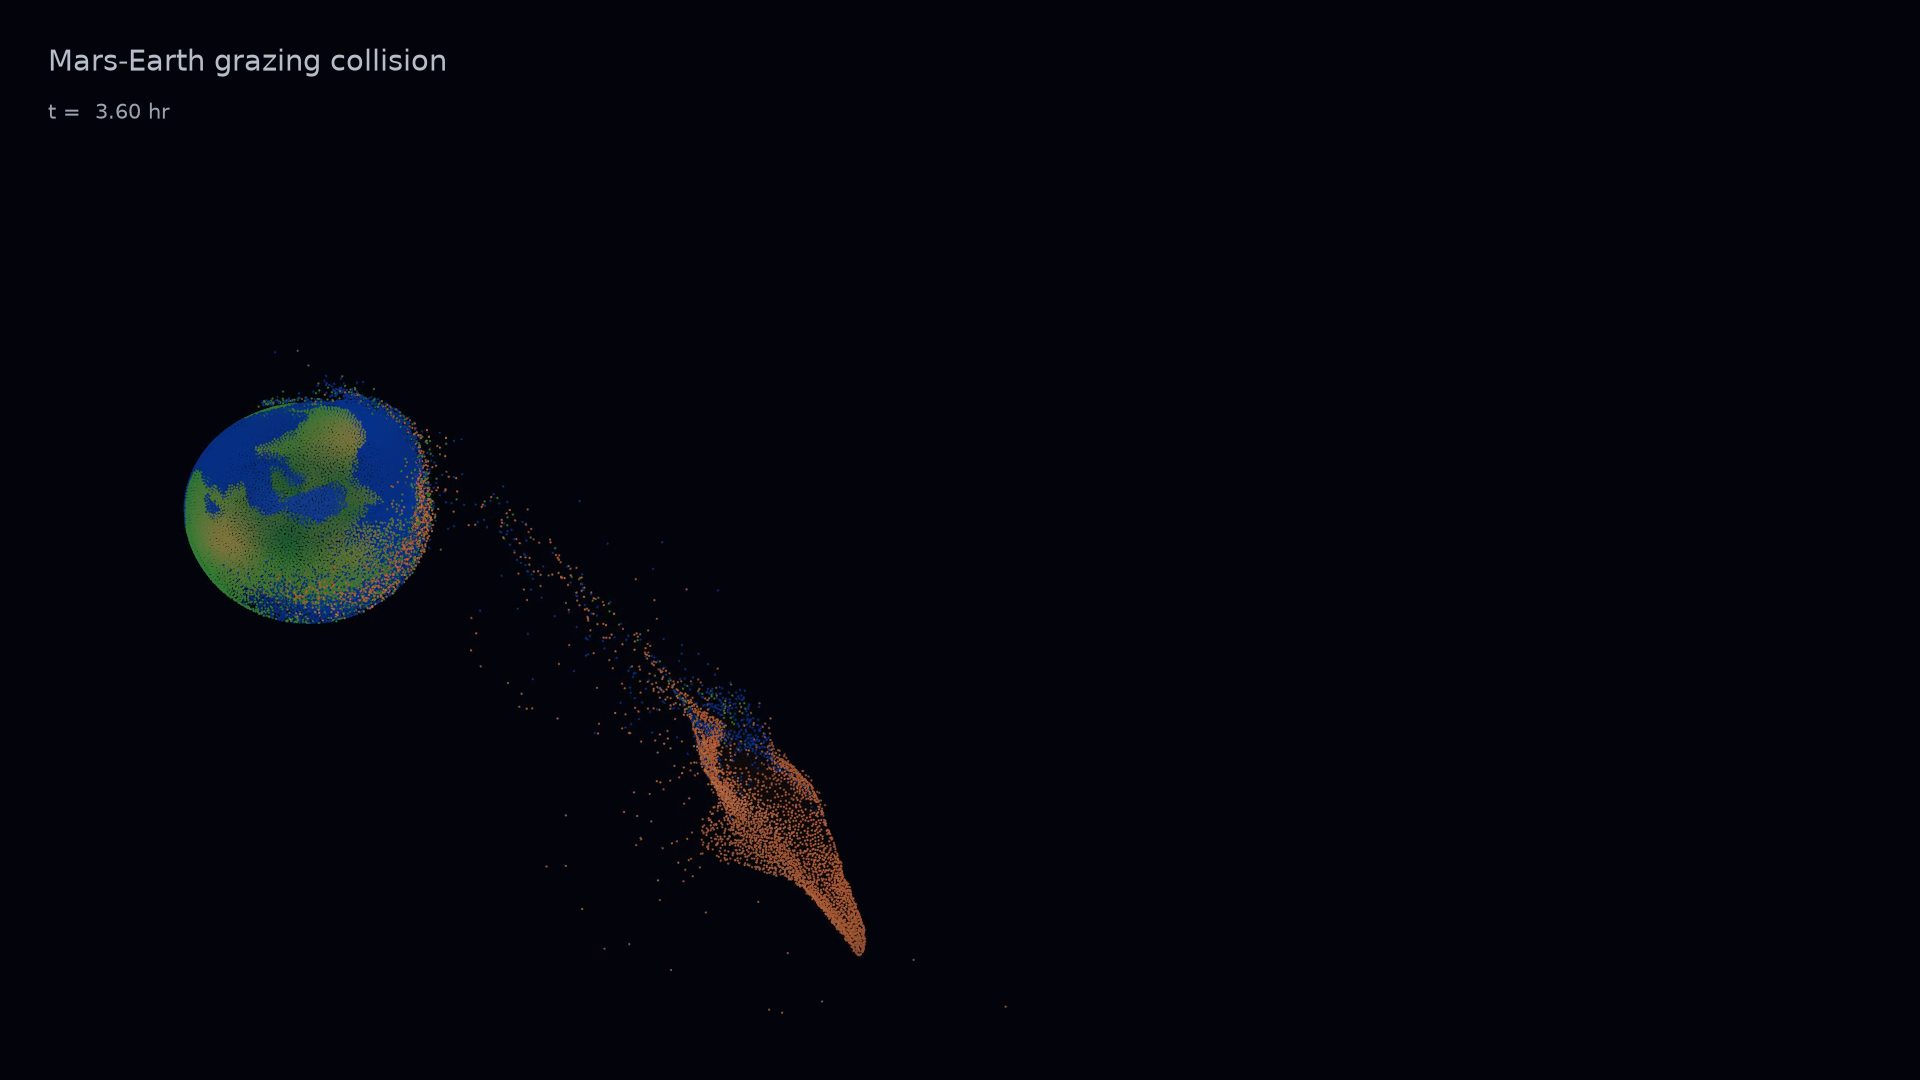
\includegraphics[width=0.49\textwidth]{../docs/figures/direct_view_02_contact.png}
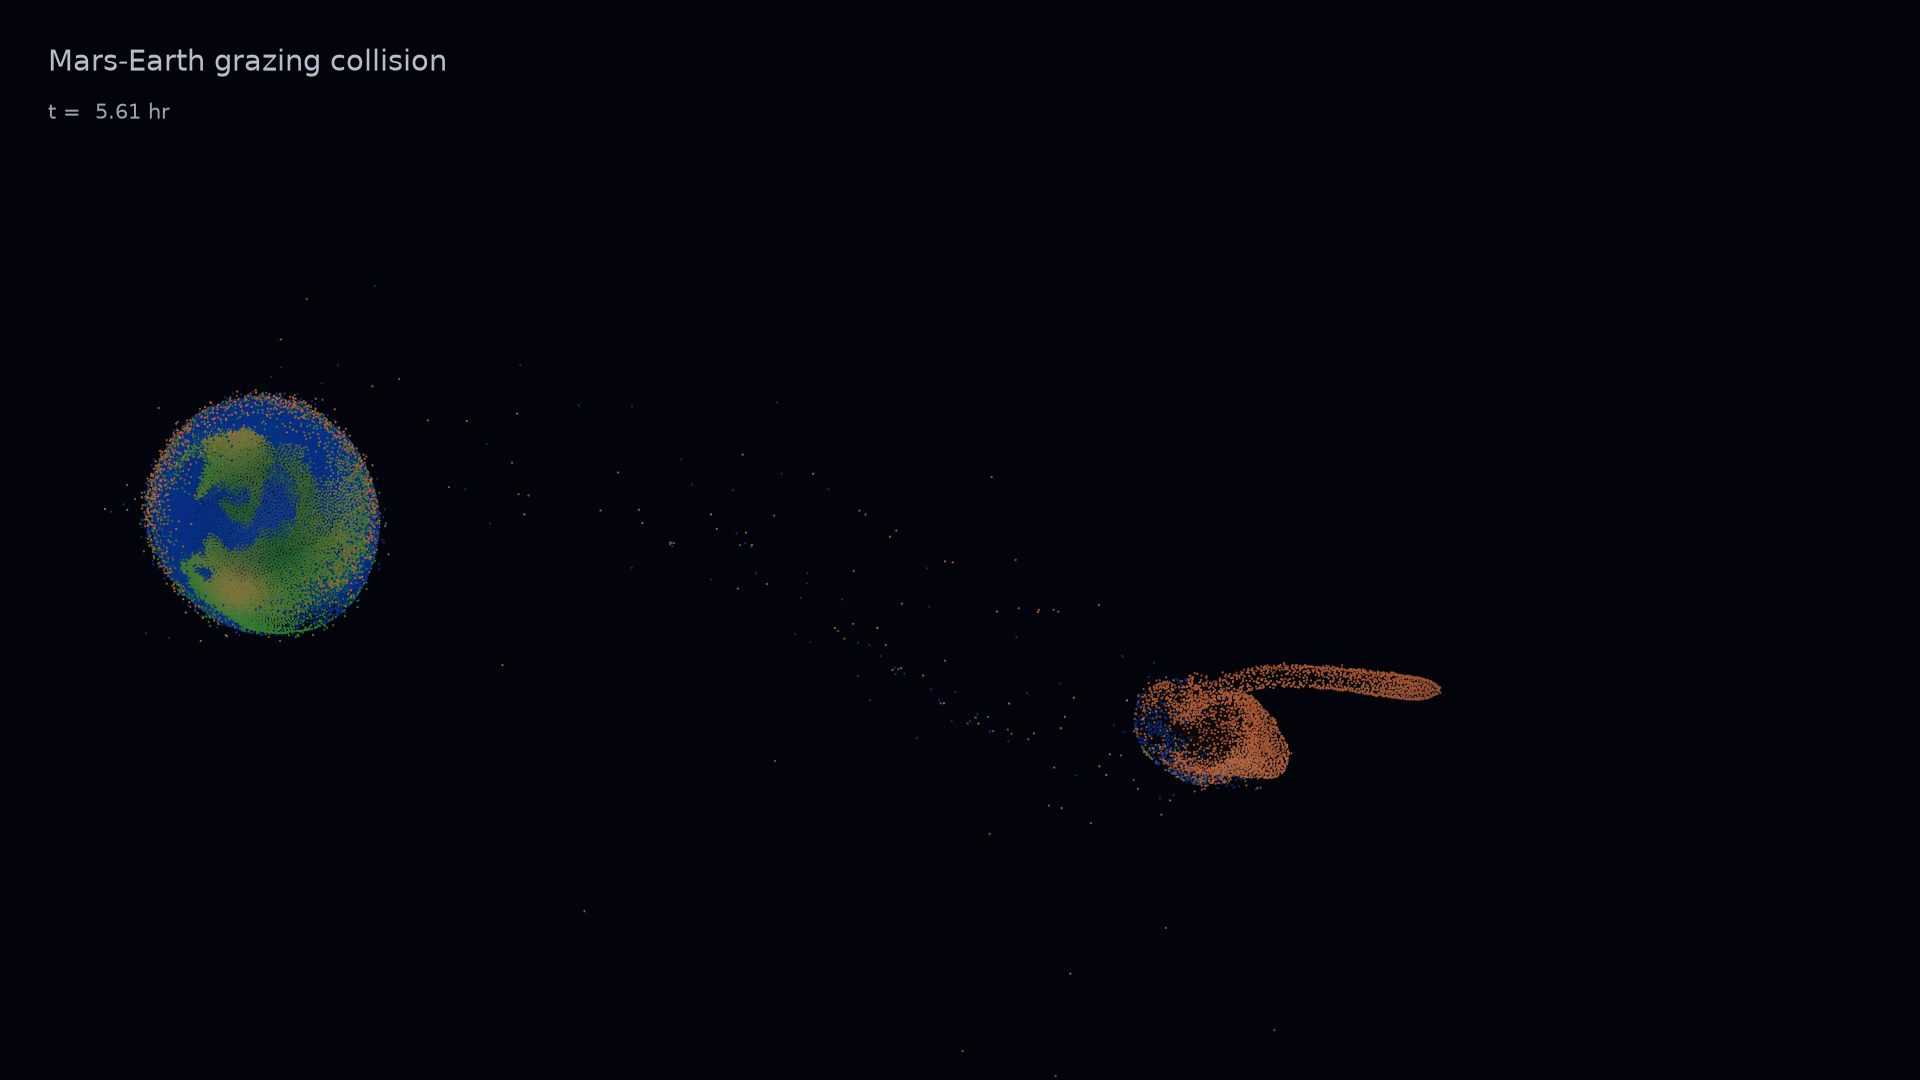
\includegraphics[width=0.49\textwidth]{../docs/figures/direct_view_03_departure.png}
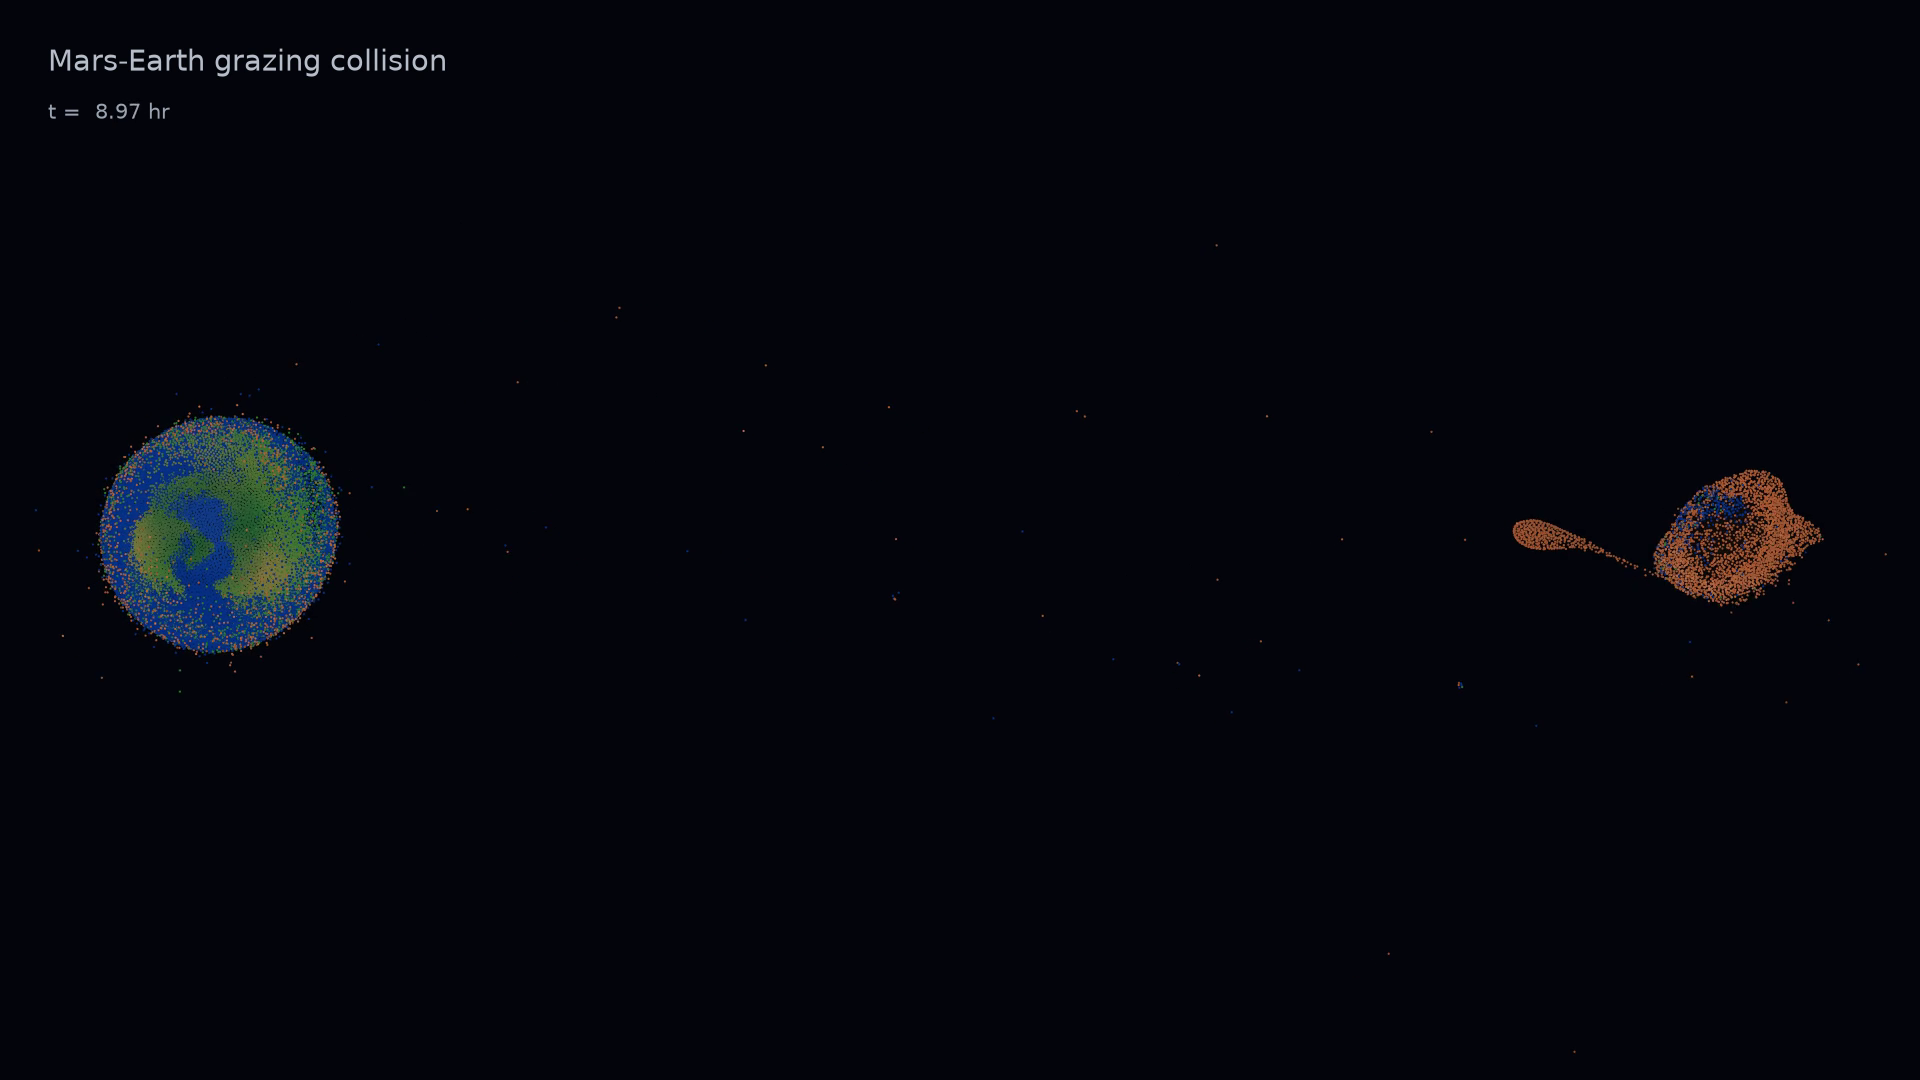
\includegraphics[width=0.49\textwidth]{../docs/figures/direct_view_04_final.png}
\caption{Selected frames from the inertial-frame direct-view render.  The
panels show the initial configuration, close interaction, departure, and final
nine-hour state.  The surface colors are tracer labels advected with SPH
particles, not texture maps pasted onto a rendered sphere.}
\label{fig:direct_frames}
\end{figure*}

\section{Current Outcome}

The first passage is strongly grazing rather than a direct head-on merger.  The
Mars-mass impactor is tidally elongated and partially stripped, transfers
material to the Earth remnant and debris stream, and initially departs as a
coherent Mars-rich remnant.  A compact Mars-derived secondary is identifiable by
36 hours, but point-mass integrations initialized from that state predict
Roche/contact-scale passages and therefore cease to be reliable before the next
encounter.

The hydrodynamic continuation confirms that a serious second finite-size
encounter occurs.  It produces a long tidal/accretion stream and substantial
rearrangement of the visible clumps.  The 92-hour endpoint has not yet received a
full particle-binding and source-material census, so visual compactness alone is
insufficient to label a permanent satellite, merger, survivor, or escaping body.
The robust conclusion from this realization is renewed hydrodynamic interaction,
not a final outcome classification.

\section{Limitations and Required Publication Work}

Several steps remain before this workflow can support publication-quality
physical conclusions.  The completed 20k--200k visualization ladder must be
analyzed quantitatively and extended around the second encounter; a single
200k-particle realization is low by the standards of detailed giant-impact
outcome studies.  Conservation diagnostics must be reported systematically:
total energy, angular momentum, linear momentum, particle removal, mass
partitioning, and thermodynamic state should be tracked across every continuation
boundary.  The final snapshot and preceding checkpoints require a persistent-ID
clump and debris census.  The initial thermal profile, differentiated structure,
equation of state, relaxation procedure, spin, impact angle, and velocity must be
varied before assigning an outcome boundary.

The rendering pipeline also imposes interpretive choices.  Surface tracers are
faithfully advected particle labels, but the land/ocean and Mars albedo maps
are visual encodings, not resolved geology.  The density-layer trial renderer
uses the SPH smoothing lengths to create a projected semi-transparent field,
which is useful for seeing interiors and debris curtains but is still a
visualization product rather than a radiative-transfer calculation.

\section{Reproducibility}

The GitHub repository stores the scripts, compact initial-condition files,
sidecar labels, YAML configuration files, selected diagnostics, rendered movies,
and quality-control stills.  The largest generated snapshot directories and
continuation logs are not stored directly in Git; they are documented in
\texttt{manifests/LARGE\_ARTIFACTS.md}.  Recreating the full rendered sequence
requires the SWIFT and WoMa environments documented in the repository, the
corresponding snapshot time series, and the renderer commands recorded in the
README and scripts.

\section{Summary}

We have assembled a reproducible workflow and a 92-hour SPH realization of a
Mars--Earth grazing collision.  The calculation combines differentiated settled
bodies, advected surface tracers, an initial grazing passage, a later finite-size
encounter, and presentation-oriented render products.  It is appropriate as a
scientifically informed animation asset and as a foundation for a quantitative
study.  Publication-quality outcome claims require a final binding census, an
explicit conservation audit, and a broader resolution and parameter survey.

\acknowledgments
This draft was prepared as documentation for a local scientific-visualization
project.

\software{SWIFT, WoMa, SEAGen, Python, NumPy, SciPy, h5py, Matplotlib, FFmpeg}

\end{document}
